\appendix
\section{Artifact Appendix}

Checklist: commands are run from the repo root. Each step has a machine-checkable PASS condition.

\begin{enumerate}
\item \textbf{Unit/regression suite}
\begin{verbatim}
python -m pytest -q
\end{verbatim}
\textit{Expected:} exit code \texttt{0} (PASS).

\item \textbf{Software gate (self-audit)}
\begin{verbatim}
python tools/audit_min.py --mode software
\end{verbatim}
\textit{Expected (PASS):}
\begin{itemize}
\item exit code \texttt{0}
\item JSON contains \texttt{decision == \"GO\"}
\item criteria include (as documented in the artifact index):
\begin{itemize}
\item \texttt{dslReady: True}
\item \texttt{digestMatchAll: True}
\item \texttt{benchVerifyOk: True}
\item \texttt{b3Evidence302\_7500: True}
\item \texttt{graphCountsNormalized: True}
\end{itemize}
\end{itemize}

\item \textbf{Bit-exactness verifier for core benchmarks (golden \texorpdfstring{$\\leftrightarrow$}{<->} C++ reference)}
\begin{verbatim}
python -m nema bench verify benches/B1_small/manifest.json --outdir build/paper_verify/b1
python -m nema bench verify benches/B3_kernel_302_7500/manifest.json --outdir build/paper_verify/b3
\end{verbatim}
\textit{Expected (PASS) for each run:}
\begin{itemize}
\item the verifier JSON reports:
\begin{itemize}
\item \texttt{ok == true}
\item \texttt{mismatches == []} (mismatch = 0)
\item (if exposed) \texttt{digestMatchOk == true} or equivalent
\end{itemize}
\end{itemize}

\item \textbf{External bundle workflow (B4)}
\begin{verbatim}
python -m nema bench verify benches/B4_real_connectome/manifest.json --outdir build/paper_verify/b4
\end{verbatim}
\textit{Expected (PASS):}
\begin{itemize}
\item verifier completes with \texttt{ok == true}
\item workflow expectation consistent with the spec contract: external referenced files must exist; if \texttt{sha256} is not a placeholder token, it must match the file digest.
\end{itemize}

\item \textbf{Hardware pipeline generation (HLS + Vivado evidence capture)}
\begin{verbatim}
bash tools/run_hw_gates.sh
\end{verbatim}
\textit{Expected (PASS by artifact contract):}
\begin{itemize}
\item \texttt{build\_hw/} contains at least one \texttt{**/bench\_report.json}
\item \texttt{build\_hw/} contains \texttt{**/hw\_reports/**/*.(rpt|xml|log)} (or the equivalent set consumed by the report parser)
\end{itemize}

\item \textbf{Hardware gate (self-audit)}
\begin{verbatim}
python tools/audit_min.py --mode hardware
\end{verbatim}
\textit{Expected (PASS):}
\begin{itemize}
\item exit code \texttt{0}
\item JSON contains \texttt{decision == \"GO\"}
\item criteria include (as documented in the artifact index):
\begin{itemize}
\item \texttt{hardwareToolchainAvailable: True}
\item \texttt{hardwareEvidenceG0b: True}
\item \texttt{hardwareEvidenceG2: True}
\item \texttt{hardwareEvidenceG3: True}
\item \texttt{digestMatchAll: True}
\end{itemize}
\end{itemize}

\item \textbf{Paper artifact pack sanity (pre-generated table/figure + evidence)}
\begin{verbatim}
cat papers/paperA/artifacts/tables/gates_summary.md
cat papers/paperA/artifacts/figures/gates_status.txt
\end{verbatim}
\textit{Expected (PASS):}
\begin{itemize}
\item \texttt{gates\_summary.md} shows both software and hardware with \texttt{decision = GO} (as in the artifact index preview).
\item \texttt{gates\_status.txt} exists (caption noted as missing in the artifact index; this does not affect correctness gates).
\end{itemize}

\item \textbf{Optional: checkpoint/bundle regeneration (ergonomics; not a claim)}
\begin{verbatim}
bash tools/checkpoint_full.sh
\end{verbatim}
\textit{Expected:} produces an evidence bundle and/or updated evidence directory consistent with the repository's checkpoint conventions (used to package reproducibility evidence).
\end{enumerate}

\subsection{Artifact Snapshot (pre-generated assets)}

The appendix directly references the current artifact files in \texttt{papers/paperA/artifacts/}.

\begin{figure}[h]
\centering
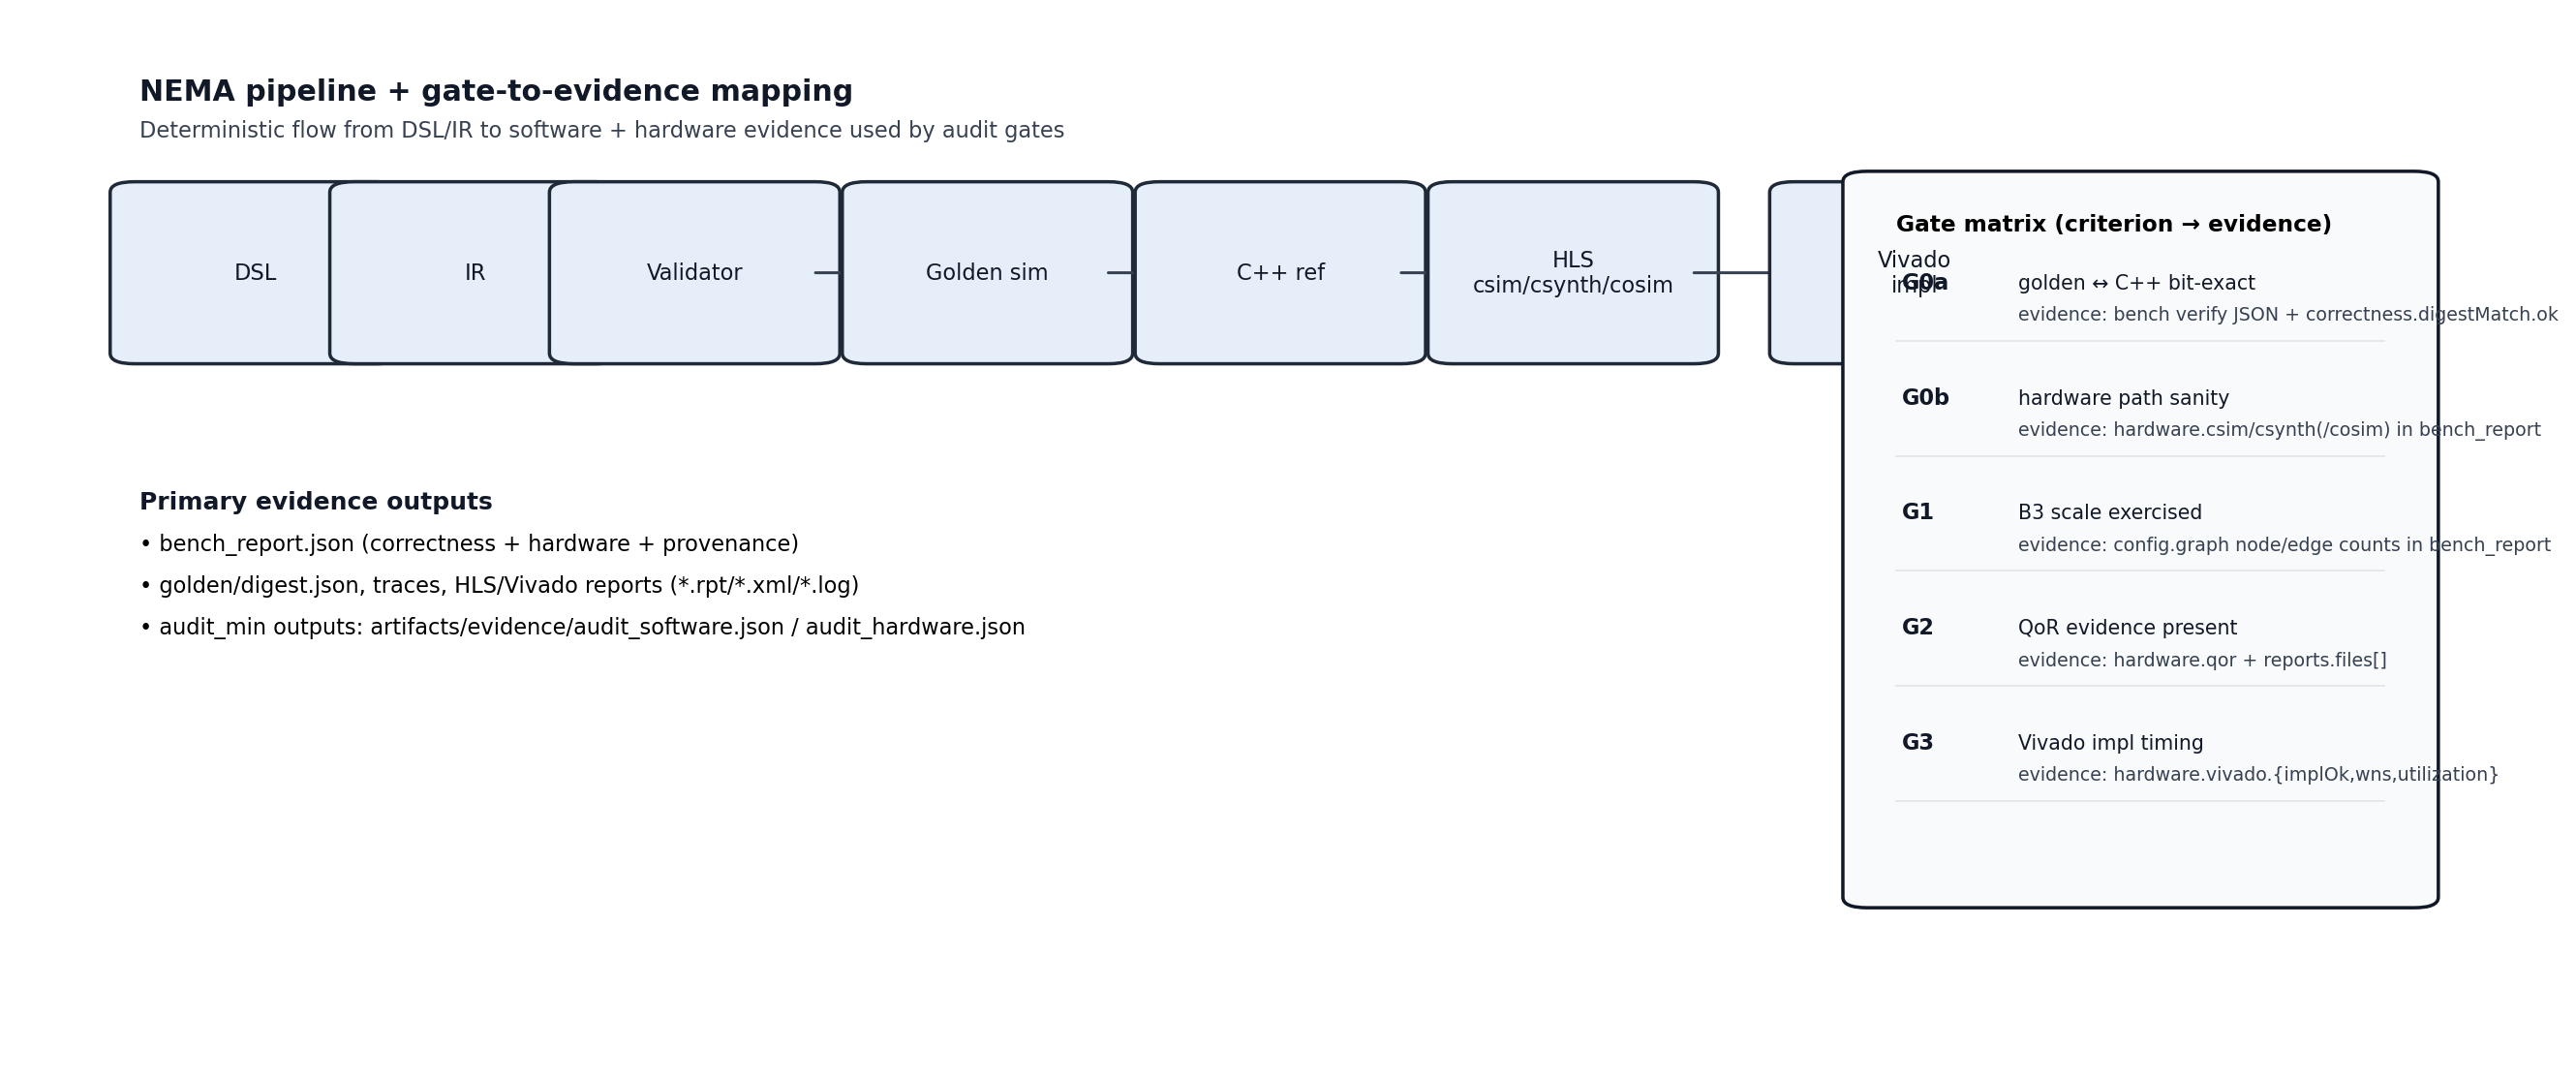
\includegraphics[width=0.98\linewidth]{../artifacts/figures/fig_pipeline_gates.png}
\caption{NEMA pipeline and gate-to-evidence mapping. G0a validates bit-exactness between golden and C++ reference (\texttt{bench verify} / \texttt{correctness.digestMatch.ok}); G0b validates hardware-path execution evidence (\texttt{csim/csynth/cosim} fields in \texttt{bench\_report.json}); G1 validates that the 302/7500 benchmark evidence is present; G2 validates QoR/report evidence (\texttt{hardware.qor} and report files); G3 validates Vivado implementation timing/utilization evidence (\texttt{hardware.vivado.*}). Gate outputs and decisions are recorded in \texttt{papers/paperA/artifacts/evidence/audit\_software.json} and \texttt{papers/paperA/artifacts/evidence/audit\_hardware.json}.}
\label{fig:pipeline-gates}
\end{figure}

\paragraph{Legacy status snapshot.}
\texttt{papers/paperA/artifacts/figures/gates\_status.txt} is retained as a lightweight artifact snapshot, but Figure~\ref{fig:pipeline-gates} is the primary evidence-facing figure used by the paper.

\paragraph{Table snapshot (\texttt{gates\_summary.csv}).}
\begin{verbatim}
mode,ok,decision,toolchainHwAvailable,software_ok,hardware_ok,all_ok
software,true,GO,True,True,True,True
hardware,true,GO,True,True,True,True
\end{verbatim}

\paragraph{Table snapshot (\texttt{gates\_summary.md}).}
\begin{verbatim}
| mode | ok | decision | toolchainHwAvailable | software_ok | hardware_ok | all_ok |
|---|---|---|---|---|---|---|
| software | true | GO | True | True | True | True |
| hardware | true | GO | True | True | True | True |
\end{verbatim}
